\documentclass{scrreprt}
\usepackage[x11names]{xcolor}	% colori
\usepackage{pgfplots}			% grafici
\usepackage{imakeidx}			% indice
\usepackage{amsfonts}			% font matematici	
\usepackage{amsthm}				% teoremi				
\usepackage{array}				% matrici
\usepackage{mdframed}			% cornici al testo
\usepackage{mathtools}			% matematica
\usepackage{hyperref}			% collegamenti ipertestuali per l'indice
\usepackage{chngcntr}			% counter per gli esercizi
\usepackage{multicol}			% colonne multiple
\usepackage[italian]{babel}

\usepackage[a4paper,
top=1cm,
bottom=1cm,
includefoot,
left=1cm,
right=1cm,
footskip=1cm]{geometry}



% Definizione dell'ambiente "Definizione"
\newtheorem{defn}{Definizione}
\newenvironment{definition}{\begin{mdframed}[backgroundcolor=Ivory2]\begin{defn}}{\end{defn}\end{mdframed}}

% Definizione dell'ambiente "Teorema"
\newtheorem{teorema}{Teorema}
\newenvironment{thm}{\begin{mdframed}[backgroundcolor=Snow2]\begin{teorema}}{\end{teorema}\end{mdframed}}

% Definizione dell'ambiente "Dimostrazione"
\newtheorem{demnstrn}{Dimostrazione}
\newenvironment{dimostrazione}{\begin{mdframed}[backgroundcolor=Snow3]\begin{demnstrn}}{\end{demnstrn}\end{mdframed}}

% Definizione dell'ambiente "Esercizio"
\newcounter{exnr}
\newtheorem{esercizio}{Esercizio}
\counterwithin*{esercizio}{section}
\newenvironment{ex}{\begin{esercizio}}{\end{esercizio}}


% Solo le equazioni referenziate vengono numerate
% vedi https://tex.stackexchange.com/a/2602
\mathtoolsset{showonlyrefs}  

\pagenumbering{gobble} % disabilita la numerazione delle pagine


\begin{document}

\section*{Indici}
\begin{itemize}
	\item ROE = Utile netto / Patrimonio netto
	\item ROA (assets) = Utile operativo / Attivo totale
	\item ROS = Utile operativo / Ricavi
	\item ROT = Ricavi / Attivo totale
	\item ROI = Utile operativo / Investimenti
	\item ROD = Oneri finanziari / debiti finanziari
	\item RA = valore produzione / capitale investito
	\item s = utile netto / utile lordo da attività in funz. ????
	\item R = oneri finanziari netti / debiti finanziari
	\item Rapporto di leva = mezzi di terzi / patriomonio netto
	\item autonomia finanziaria = patrimonio netto / attivo totale
	\item elasticità ai finanziamenti = passività correnti / totale attivi
	\item rapporto corrente = attivo corrente / passivo corrente
	\item Equilibrio medio-lungo = CF operativo / passività non correnti
	\item MON = margine operativo netto = utile operativo - oneri finanziari
	\item MLI = margine lordo industriale = ricavi - costi pieni industriali
	\item D/E = debiti finanziari / patrimonio netto
	\item RC = attivo corrente / passivo corrente $\leftarrow$ indice liquidità
	\item TA = attivo corrente - rimanenze / passivo corrente $\leftarrow$ indice liquidità
\end{itemize}

\subsection*{Analisi}
ROI $>$ ROD significa gestione efficace e efficiente.\\
D/E $>$ 1 significa che l'azienda ha più debiti che patrimonio netto. Molto rischioso se $>$ 2.\\
RA misura produttività del capitale.\\

\section*{Contabilità analitica (costing)}

\subsection*{Job order costing o process costing o activity based costing}
Se ho produzione a flusso continuo uso process costing, altrimenti job order costing.\\
Se ho produzione a flusso continuo e produco prodotti diversi uso activity based costing.\\
Job order costing: calcolo il costo per ogni ordine di produzione.\\
Process costing: calcolo il costo per ogni fase di produzione.

\subsection*{Più reparti}
\begin{enumerate}
	\item Scrivo bene tutte le informazioni
	\item Studio consumo per ogni fase: Materie prime, elettricità ecc
	\item Attenzione a capire cosa si consuma in base alla percentuale di lavorazione
	\item WIP e prodotto dello stesso tipo vanno separati
\end{enumerate}
CPA = CPI + costi periodo\\
MLI = fatturato - costo del venduto\\
dove:
\begin{itemize}
	\item CC = costo conversione = costo lavoro diretto + overhead
	\item CPA = costi pieno aziendale = CPI + costi costi di periodo
	\item CPI = costi pieno industriale = CC + costi materiali diretti (MD)
	\item MLI = margine lordo industriale = fatturato - CPI
\end{itemize}

\subsection*{Un solo reparto}
\begin{enumerate}
	\item Per ogni reparto calcolo: \begin{enumerate}
		\item MD: costo materie prime + costo materiale di consumo
		\item LD: costo lavoro diretto
		\item OVH: overheads (costi indiretti tipo ammortamenti/elettricità)
	\end{enumerate}
	\item Calcolo il costo pieno industriale (CPI) = MD + LD + OVH
	\item Calcolo CPI\textsubscript{u} = CPI / quantità prodotta
\end{enumerate}

\section*{Decisioni a breve termine (make or buy / mix / break-even)}
\subsection*{Make or buy}
\begin{enumerate}
	\item Scegliere se conviene comprare o produrre internamente
	\item Calcolo costo di acquisto (prezzo unitario * quantità)
	\item Calcolo costo di produzione (Somma MD + LD + OVH)
	\item Scelgo il minore
\end{enumerate}

\subsection*{Break-even}
per il break even point calcolo i costi fissi e li divido per il margine di contribuzione unitario (prezzo - costo variabile unitario).\\
Se voglio fare break even a un certo MON (margine operativo netto) , al costo fisso aggiungo il MON e divido per il margine di contribuzione unitario.

\subsection*{Mix}
Verifico se riesco a produrre i prodotti fino a saturare la domanda o se ho vincoli di produzione.\\
Se ho vincoli di produzione, calcolo il margine di contribuzione unitario e lo divido per il tempo di produzione (del vincolo). Produrrò prima i prodootti con il maggiore rapporto MCU/tempo di produzione.\\
Se ho penale, sviluppo i casi(produco meno x/meno y/meno x): in ogni caso calcolo il margine totale e scelgo il caso migliore.


\section*{investimenti}
WACC = (patrimonio netto / capitale investito) * costo del capitale + (debiti finanziari / capitale investito) * costo del debito * (1 - aliquota fiscale)\\
Colonne tabella:
\begin{itemize}
	\item Ricavi
	\item Costi variabili
	\item Imponibile (ricavi - costi variabili)
	\item Ammortamenti / plusvalenze / minusvalenze
	\item Imponibile per tasse (imponibile - ammortamenti)
	\item Tasse (imponibile per tasse * aliquota)
	\item Flusso cassa lordo (imponibile - tasse)
	\item investimenti (segno negativo)
	\item flusso di cassa netto (flusso cassa lordo + investimenti)
	\item Flusso di cassa netto attualizzato (FCN / (1 + tasso)\textsuperscript{periodo})
\end{itemize}

Se devo scegliere tra due investimenti, calcolo il VAN (valore attuale netto) e scelgo quello con VAN maggiore.\\
Se devo scegliere tra la situazione attuale e un investimento, calcolo il TIR (tasso interno di rendimento) e se è maggiore del tasso di riferimento, scelgo l'investimento. In alternativa, calcolo il van considerando i delta di costi/ricavi/investimeno e investo se il VAN è maggiore di zero.\\

Calcolo il payback time: calcolo il flusso di cassa netto cumulato e vedo quando diventa positivo.\\
Calcolo Profitability index: VAN / investimento. Se è maggiore di 1, l'investimento è conveniente.\\
Calcolo TIR: $\sum_{t=0}^{n} \frac{FCN_t}{(1 + TIR)^t} = 0$ con $FCN_t$ flusso di cassa netto al tempo t.\\


\section*{Organizzazione aziendale}
\subsection*{Struttura organizzativa}
Span: numero di dipendenti che un manager può gestire, ovvero numero di blocchi immediatamente inferiori.\\
Depth: numero di livelli gerarchici. Attenzione a contare bene i livelli, il disegno può confondere.\\

\subsection*{Specializzazione}
Specializzazione orizzontale: si riferisci al modo in cui i compiti sono ripartiti.\\
Specializzazione verticale: indica la separazione tra compiti di coordinamento e compiti operativi, ovvero tra manager e maker. Se sei molto controllato, alta specializzazione verticale.\\

Esempio: azienda 2 dipendenti, clienti privati o imprese, funzione di sales o service.\\
Se un dipendente fa privati e l'altro imprese, bassa specializzazione orizzontale.\\
Se un dipendente fa sales e l'altro service, alta specializzazione orizzontale.\\

\subsection*{Tipi di organizzazione}
\begin{itemize}
	\item Struttura semplice (tutti fanno tutto / bassa formalizzazione)
	\item Struttura funzionale: dipendenti divisi per funzioni
	\item Struttura divisionale: dipendenti divisi per divisioni(geografiche / di mercato / di prodotto)
	\item Struttura ibrida
	\item Struttura matriciale: dipendenti divisi per funzioni e divisioni
\end{itemize}

\section*{Mercato}
Elasticità della domanda al prezzo: $\epsilon_x = \left\lvert \frac{\delta q_x}{\delta p_x} \frac{p_x}{q_x}\right\rvert$\\
Nel monopolio, condizione di massimo profitto: $\frac{p(q)-CM(q)}{p(q)} = \frac{1}{\epsilon}$ con CM costo marginale.




\section*{Bilancio}
Stato patrimoniale:

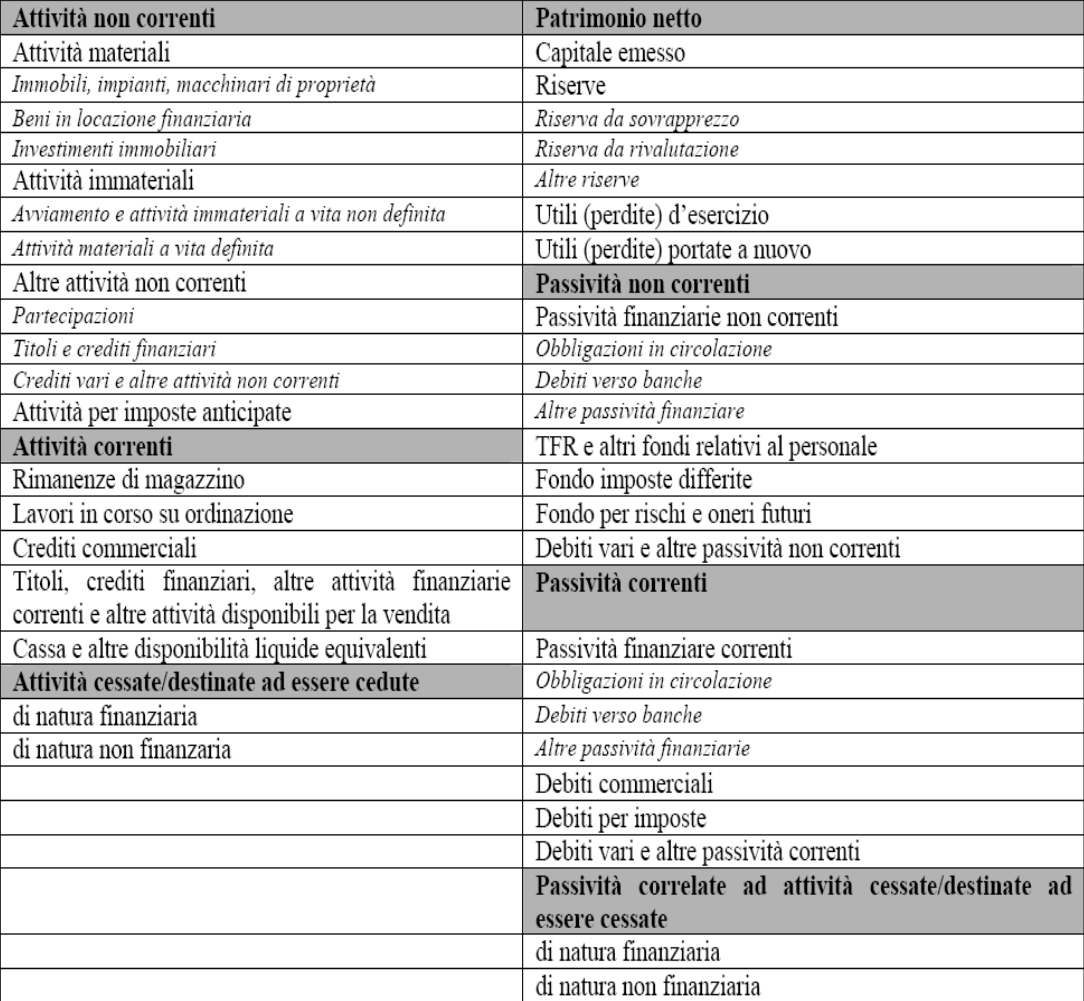
\includegraphics[scale = 0.3]{stato_pat.png}

Conto economico:

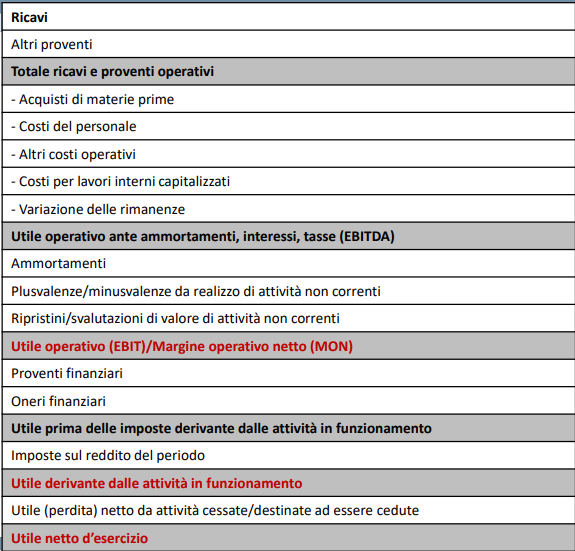
\includegraphics[scale = 0.5]{conto_eco.png}

Rendiconto finanziario indiretto:

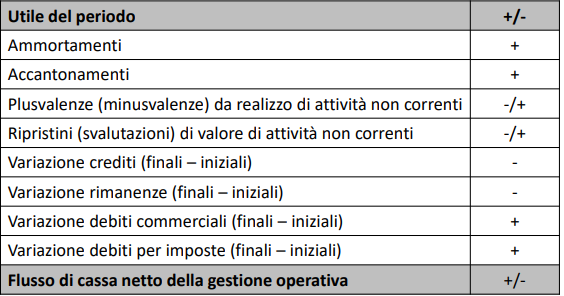
\includegraphics[scale = 0.5]{rend_fin_ind.png}

Rendiconto finanziario diretto:

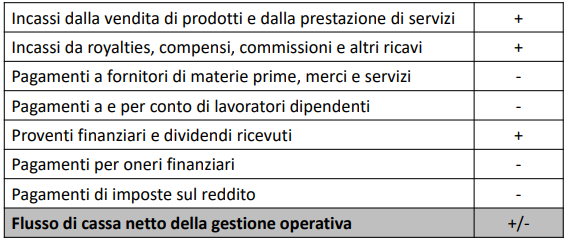
\includegraphics[scale = 0.5]{rend_fin_dir.png}

\end{document}